\chapter{Energy}

\section*{Level of clean energy capacity (megawatts) installed as a result of International Climate Finance (ICF) support.}

\thispagestyle{empty}



\section{Results}

From 2015/16 to 2019/20 DFID installed \textbf{
771
} of clean energy capacity (Table \ref{tab:energy}). %

\begin{figure}[htbp]
	\centering
\begin{knitrout}
\definecolor{shadecolor}{rgb}{0.969, 0.969, 0.969}\color{fgcolor}
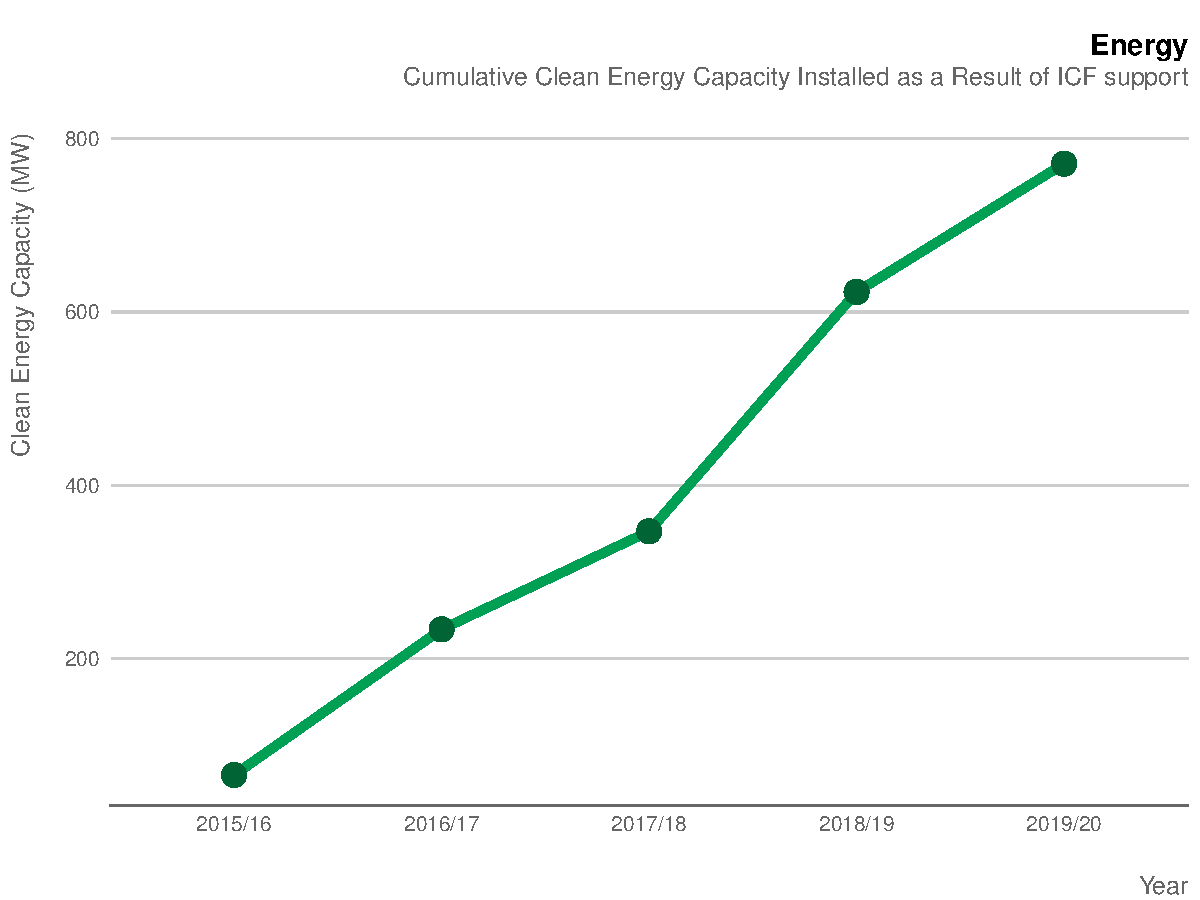
\includegraphics[width=0.8\textwidth]{figs/energy_cumulative_plot-1} 

\end{knitrout}
	%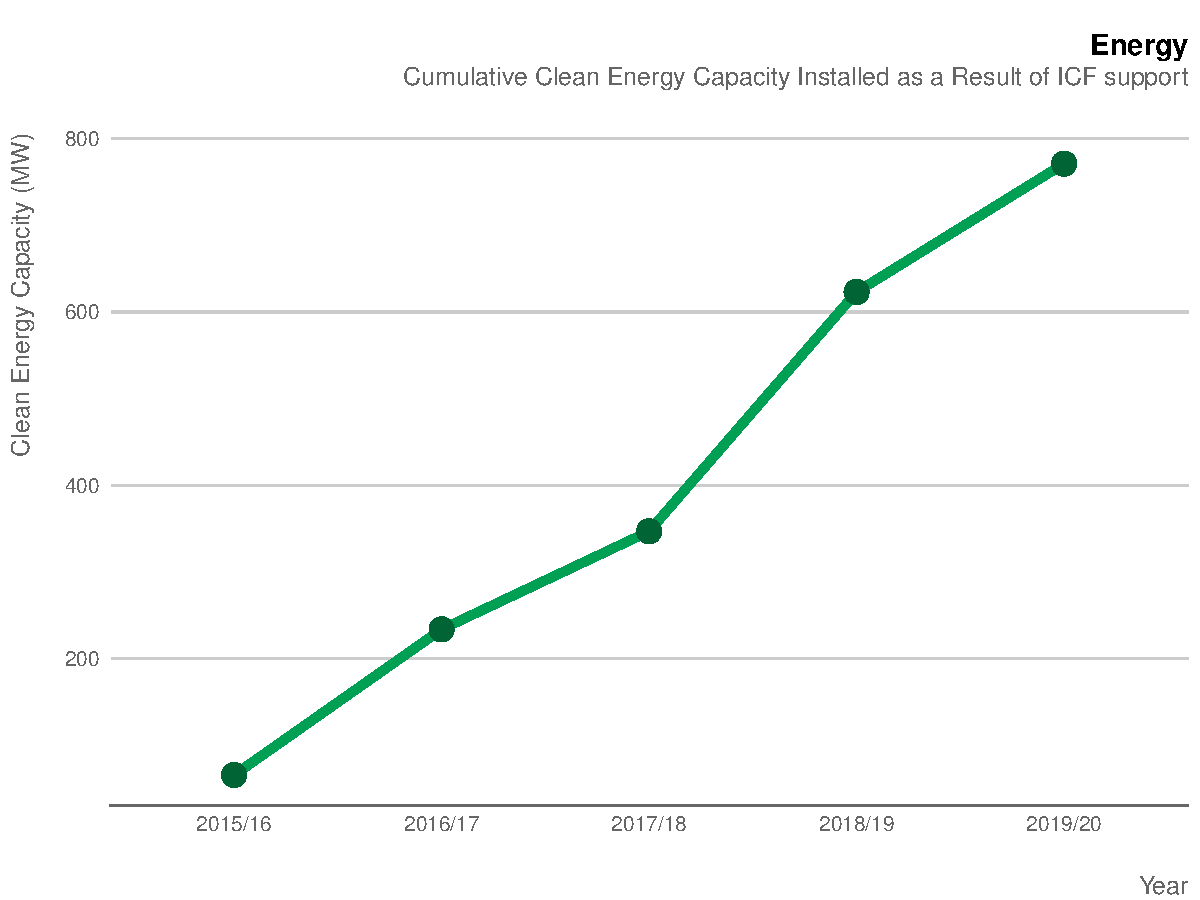
\includegraphics[width=0.7\textwidth]{../figs/energy_cumulative_plot} \hfill
	\caption{Line plot of cumulative clean energy capacity installed (in megawatts) from 2015/16 to 2019/20.}
	\label{fig:energy_cumulative_plot}
\end{figure}

When new information becomes available, historic estimates are updated during each annual results reporting round to reflect the best available information on programme achievements. %
As a result, several corrections to past years' data have been made this year. %
A number of programmes, which DFID has supported for multiple years, have reported results for the first time leading to an increase in historic results. %
Simultaneously, corrections were made to results estimates from the Clean Technology Fund (CTF), following a review by government analysts and the Climate Investment Fund's (CIFs) audit unit.  %
Corrections have been made where it was discovered that either results were being taken from the wrong source, data were inputted incorrectly, or inappropriate adjustments for over/under reporting had been made. %
These errors are difficult pick up during the quality assurance process since the CIFs rely on implementing partners to report project data accurately in the first instance. %

% Need to convert to xtable
\begin{table}[htbp]
	\centering
  \caption{Cumulative Totals of MW Clean Energy Capacity Installed (ICF KPI 7)}\label{tab:energy}
	\begin{tabular}{rrrrr}
		\toprule
		\multicolumn{1}{c}{\textbf{2015/16}}&\multicolumn{1}{c}{\textbf{2016/17}}&\multicolumn{1}{c}{\textbf{2017/18}}&\multicolumn{1}{c}{\textbf{2018/19}}&\multicolumn{1}{c}{\textbf{2019/20}} \\ \hline
		\rule{0pt}{10pt}66 	  &      234 	&        347 	   &     623 	  &        771 \\ \bottomrule
	\end{tabular}
\end{table}

\section{Context}

This indicator measures clean energy capacity installed as a result of DFID
programming. %

Access to energy is a constraint to inclusive economic growth and job creation across all of DFID's focus countries. %
Population growth is also pushing up energy demand; investments in electricity generation, transmission and distribution and connections have failed to keep pace. %
In our economic development strategy we made clear we will adopt a `climate smart' approach across our economic development work --- including through sustainable energy. %
We are working to help meet businesses' rising energy needs; to ensure affordable energy access for the poor; and to enhance environmental sustainability in energy use. %


\newpage
